
\documentclass[preprint,11pt]{elsarticle}
\biboptions{sort&compress}
%% Use the option review to obtain double line spacing
%% \documentclass[preprint,review,12pt]{elsarticle}

%% Use the options 1p,twocolumn; 3p; 3p,twocolumn; 5p; or 5p,twocolumn
%% for a journal layout:
%% \documentclass[final,1p,times]{elsarticle}
%% \documentclass[final,1p,times,twocolumn]{elsarticle}
%% \documentclass[final,3p,times]{elsarticle}
%% \documentclass[final,3p,times,twocolumn]{elsarticle}
%% \documentclass[final,5p,times]{elsarticle}
%% \documentclass[final,5p,times,twocolumn]{elsarticle}

%% The graphicx package provides the includegraphics command.
%\usepackage{graphicx}
%% The amssymb package provides various useful mathematical symbols
\usepackage{amssymb}
%% The amsthm package provides extended theorem environments
%% \usepackage{amsthm}

%% The lineno packages adds line numbers. Start line numbering with
%% \begin{linenumbers}, end it with \end{linenumbers}. Or switch it on
%% for the whole article with \linenumbers after \end{frontmatter}.
\usepackage{lineno}

%% natbib.sty is loaded by default. However, natbib options can be
%% provided with \biboptions{...} command. Following options are
%% valid:

%%   round  -  round parentheses are used (default)
%%   square -  square brackets are used   [option]
%%   curly  -  curly braces are used      {option}
%%   angle  -  angle brackets are used    <option>
%%   semicolon  -  multiple citations separated by semi-colon
%%   colon  - same as semicolon, an earlier confusion
%%   comma  -  separated by comma
%%   numbers-  selects numerical citations
%%   super  -  numerical citations as superscripts
%%   sort   -  sorts multiple citations according to order in ref. list
%%   sort&compress   -  like sort, but also compresses numerical citations
%%   compress - compresses without sorting
%%
%% \biboptions{comma,round}

% \biboptions{

%   --------------------------------------------------------------------
%       Text dimensions
%   --------------------------------------------------------------------
\usepackage[dvips]{geometry}
\geometry{letterpaper,left=3.0cm,right=2.0cm,top=3.0cm,bottom=2.0cm}


\usepackage{adjustbox}
\usepackage{graphicx}
\usepackage{subfigure}
\usepackage[cmex10,fleqn]{amsmath}
\usepackage{nccmath}
\usepackage{algorithmic}
\usepackage{array}
%\usepackage[colorlinks=true,citecolor=blue,linkcolor=blue,urlcolor=blue,plainpages=false]{hyperref}
\usepackage[bookmarks=false,pdfstartview={FitH},colorlinks=true,citecolor=black,linkcolor=black,urlcolor=black,plainpages=false]{hyperref}
\usepackage{breakurl}
\usepackage{nomencl}
\usepackage{multirow}
\usepackage{multicol}
\usepackage{stfloats}
\usepackage{mdwmath}
\usepackage{mdwtab}
\usepackage{eqparbox}
\usepackage{amsfonts}
\usepackage{amsbsy}
\usepackage[dvipsnames]{xcolor}
\usepackage{graphicx}
\usepackage{float}
\ifCLASSOPTIONcompsoc
    \usepackage[caption=false, font=normalsize, labelfont=sf, textfont=sf]{subfig}
\else
\usepackage[caption=false, font=footnotesize]{subfig}
\fi
\captionsetup[subfigure]{subrefformat=simple,labelformat=simple,listofformat=subsimple}
\renewcommand\thesubfigure{(\alph{subfigure})}
\usepackage{balance}
%\usepackage{flushend}
\usepackage{booktabs, tabularx, multirow, array,makecell}
\renewcommand\theadfont{\normalfont}
\usepackage{ragged2e}
\newcolumntype{Y}{>{\hsize=1.75\hsize}X}
\newcolumntype{Z}{>{\hsize=.875\hsize\RaggedLeft}X}
\setlength\extrarowheight{1.5pt}
\usepackage{pifont}
\newcommand{\B}[1]{\textcolor{black}{#1}}
\newcommand{\R}[1]{\textcolor{red}{#1}}

\usepackage[spanish]{babel} % Para soporte en español
\usepackage{graphicx} % Para manejar imágenes
\usepackage[spanish]{caption} % Asegúrate de cargar caption con la opción español

\usepackage[style=numeric, backend=biber]{biblatex}
\addbibresource{referencias.bib}


\begin{document}

\begin{frontmatter}

\title{Modelo de despacho y asignación de buses}


%% Group authors per affiliation:
\author[label1]{Martin Del Gordo}
\address[label1]{Departamento de Ingenier\'ia Industrial, Universidad de Los Andes, Colombia}
\ead{m.delgordo@uniandes.edu.co}

\author[label1]{Samuel Rubio}
\ead{s.rubioc2@uniandes.edu.co}

\author[label1]{Javier Barrera}
\ead{j.barrerahu@uniandes.edu.co}





\end{frontmatter}

\linenumbers
\section{Introducción}
\vspace{-1mm}
\label{Int}

El despacho eficiente de buses es un componente crítico en la gestión de sistemas de transporte público. La optimización del despacho busca principalmente mejorar la puntualidad, reducir los tiempos de espera de los pasajeros y minimizar los costos operativos de las empresas de transporte, entre otros. A pesar de los avances en la planificación del transporte público, muchas regiones aún enfrentan desafíos significativos en la sincronización y distribución de buses, lo cual puede derivar en servicios ineficientes y poco confiables. Los modelos tradicionales de despacho de buses suelen basarse en horarios fijos o reglas simples, que no siempre responden a las variaciones en la demanda de pasajeros o las condiciones del tráfico. Estas aproximaciones pueden resultar en una utilización ineficiente de los recursos, bien sea por un exceso o una falta de vehículos en ciertos momentos del día. Por lo tanto, existe una necesidad urgente de desarrollar modelos más sofisticados que permitan una asignación dinámica y optimizada de buses, adaptándose en tiempo real a las fluctuaciones en la demanda y otras condiciones operativas. En los últimos años, la investigación en la optimización del despacho de buses ha avanzado considerablemente gracias a la integración de técnicas de modelado matemático y algoritmos de optimización. Los enfoques más recientes han incorporado modelos de optimización basados en la programación lineal, algoritmos heurísticos y métodos metaheurísticos como algoritmos genéticos y optimización por enjambre de partículas. Estos modelos buscan equilibrar múltiples objetivos, como la minimización de los tiempos de espera de los pasajeros, la reducción de las emisiones de carbono y la mejora de la confiabilidad del servicio. 

Este problema se puede entender desde dos puntos de vista, desde el punto de vista de los usuarios y de las empresas. Las empresas generalmente buscan minimizar costos, maximizar utilidades, tener buena frecuencia de buses donde en algunos casos se terminan olvidando de las necesidades de los usuarios y se enfocan más en los objetivos empresariales. Mientras que los usuarios solo buscan tener un buen medio de transporte, facilidad, comodidad entre otros elementos. Esto muestra que tener una solución para ambas entidades sea muy complicado. 

 


\section{Estado del Arte}
\vspace{-1mm}
\label{Int}
Usualmente, los problemas de medios de transporte público se dividen en cinco diferentes tipos de objetivos. El primer tipo de problema es el diseño de rutas, este problema se centra en planificar y definir las distintas rutas de transporte público con el objetivo de satisfacer las necesidades de los usuarios y al mismo tiempo las de la empresa. Segundo, la frecuencia de los buses para generar satisfacción en los clientes. Tercero el horario de cada ruta y la salida de los buses para mantener un sistema estable en el medio de transporte. Cuarto, la programación de los distintos tipos de vehículos en el sistema, y, por último, la programación de los empleados, quienes son responsables de que el sistema funcione . Cada uno de estos objetivos cuenta con distintos supuestos necesarios para llegar a una solución, lo que contribuye a que el sistema de transporte público sea multiobjetivo, dificultando el análisis y las diversas soluciones.

Estos problemas son de gran complejidad y, cada año, con el avance de la tecnología, se obtienen respuestas más rápidas y mejores. Sin embargo, la solución de un sistema de transporte, aunque se aborde desde distintas perspectivas, sigue siendo considerada un problema NP-Hard (Magnanti, 1984)\cite{magnanti1984}. Un problema NP-Hard, o problema NP-duro, es aquel cuya complejidad es tal que no se puede reducir el tiempo de obtención de resultados. Estos problemas son tan difíciles de resolver que no existen algoritmos que puedan resolverlos en tiempo polinómico.

El primer tipo de problema que se plantea es el diseño de las rutas o en ingles \textit{Transit network design (TNDP). }El objetivo de este problema es determinar las rutas en las cuales los distintos buses van a operar con sus respectivas paradas. La solución de este tipo de problema normalmente hace uso de la matrices origen destino donde se busca satisfacer toda la población o mayor parte de la población. Este problema tiene distintas posibles restricciones para su solución, uno de los autores (Murray 2003) \cite{murray2003}  que plantean la solución es mencionando distintas características como la cobertura de las rutas, longitud de rutas, densidad y la parada de los buses. Por otro lado (Murray 1998)  \cite{murray1998} utiliza el supuesto de la satisfacción de la demanda la cual debe ser superior al 90\% teniendo en cuenta los tipos de buses, las rutas y sus longitudes. Por lo cual de esta forma evidenciamos distintos factores importantes que se pueden utilizar para solucionar un problema TNDP. Estos factores pueden ser el tipo de bus, la longitud, densidad, cantidad de paradas de buses y la demanda. 

El segundo tipo de problema es la frecuencia de los buses o en ingles \textit{Transit network frequencies settings} o con sus iniciales un problema (TNFSP). Este problema trata de establecer la frecuencia de cuantas veces pasan los buses en rutas ya establecidas. El problema TNFSP hace uso de rutas ya establecidas, y con estas rutas cumplir con la capacidad de cada tipo de bus, la satisfacción de la demanda, el número de rutas y la cantidad de buses. De esta forma se conoce la cantidad de veces que se pasa por una ruta. Donde distintos autores para encontrar la frecuencia establecen distintos objetivos, desde la mayor satisfacción de la demanda o minimizar los costos de operación. 

El tercer tipo de problema que se tiene es el problema de asignación de los horarios de los buses(despacho) o \textit{Transit network timetabling (TNTP). }Este problema como lo menciona (Valerie Guilhaire et.al 2008) \cite{guihaire2008} busca conocer la salida de los buses de una terminal o cabecera, el tiempo final de cumplir una ruta y el tiempo esperado de llegada a cada parada. Los autores mencionan que los elementos más importantes son: la satisfacción de la demanda, coordinación de transferencia, tamaño de las flotas y también el posible uso de horarios viejos ya establecidos.

El cuarto problema de la programación de los distintos buses teniendo en cuenta su frecuencia y su horario ya establecido. En otras palabras, es un problema combinado que tiene en cuenta los problemas TNTP y TNFSP. Por último, el quinto problema es la programación de empleados teniendo en cuenta la frecuencia y cada uno de los elementos de los empleados en las rutas. 

De esta forma, se evidencia la complejidad de los distintos problemas y su relación, lo que complica el entendimiento de los sistemas de transporte público. Estos problemas se pueden comprender como se muestra en el trabajo de Guihaire et al. (2008) \cite{guihaire2008} (Figura 1.). 

\captionsetup[figure]{name=Figura}
\begin{figure}[H]
  \centering
  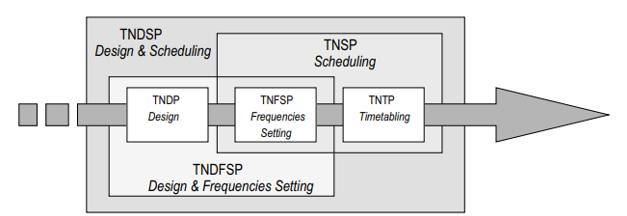
\includegraphics[width=0.8\textwidth]{tipos.png}
  \caption{Tipos de problemas en medios de transporte (Valerie Guiñhaire et.al 2008)}
  \label{fig:mi_imagen}
\end{figure}


Con el entendimiento de estos problemas se puede evidenciar el desarrollo y conocimiento del estado del arte. A continuación, se evidencia el estado del arte en los distintos tipos de problemas.

\section{Problemas en el Diseño de Redes de Transporte}

\subsection{Problema TNDP}

El problema de diseño de redes de transporte (TNDP, por sus siglas en inglés) se centra en la optimización de las rutas de los autobuses. Este tipo de problema fue identificado por primera vez en 1925 por el autor Patz, quien en su artículo (Patz, 1925)  \cite{patz1925} abordó la cuestión buscando minimizar la cantidad de asientos vacíos en los autobuses, donde el modelo estaba restringido por la capacidad del bus y la demanda del sitio. Otro autor, como (Murray 2008) \cite{murray2003}, tiene otra forma de solucionar el problema, enfocándose en establecer la cantidad de paradas en las rutas, restringido a la cobertura del sistema y el acceso disponible.

\subsection{Problema TNFSP}

El problema TNFSP, que establece la frecuencia de los buses en las rutas, es abordado por Scheele en 1980 (Scheele, 1980) \cite{scheele1980}. Su objetivo es minimizar el tiempo que los pasajeros pasan en el bus, teniendo en cuenta la capacidad del bus y la flota disponible. Por otro lado, Furth (1982) \cite{furth1982} busca maximizar el número de pasajeros y minimizar el tiempo de espera, con restricciones relacionadas con el tamaño de la flota, la espera de los buses y el presupuesto disponible.

\subsection{Problema TNTP}

El problema TNTP, propuesto por Chakroborty en 1995 \cite{chakroborty1995}, se enfoca en minimizar el tiempo total de espera de los pasajeros. Este problema utiliza el tamaño de la flota, la capacidad de la flota, el número máximo de transferencias y los tiempos de paradas como restricciones. Castelli (2004) \cite{castelli2004} trabaja en minimizar el tiempo de transferencia, considerando las rutas ya establecidas, la frecuencia disponible y el tiempo fijo entre dos buses en una ruta.

\subsection{Problema TNDFSP}

El problema TNDFSP, iniciado por Lampkin en 1967 \cite{lampkin1967}, se enfoca en el número de pasajeros directos y su tiempo total, considerando como única restricción necesaria la capacidad de los buses. Borndorfer (2005) \cite{borndorfer2005} en la ciudad de Postdam busca minimizar el tiempo de los pasajeros en las rutas y los costos, con restricciones en el cumplimiento de la demanda y el conocimiento de esta.

\subsection{Problema TNSP}

Finalmente, el problema TNSP es abordado por Eranki en 2004 \cite{eranki2004}, estableciendo las llegadas simultáneas y minimizando el tiempo de espera de los pasajeros, con la restricción de no sobrepasar el tiempo máximo de espera.

\section{Relación con el Proyecto}

Haciendo uso de lo mencionado anteriormente, se evidencian los distintos problemas en el planteamiento de un sistema de transporte público, así como las diferentes perspectivas, objetivos, supuestos y restricciones abordados por cada autor, lo que resulta en una amplia gama de soluciones.

Teniendo en cuenta estos problemas, se debe considerar el proyecto a trabajar, es un problema TNTP. El problema con Movisinu se alinea con el TNTP, ya que se busca establecer los distintos horarios de los buses de salida de la terminal para cumplir con la mayor demanda posible, generando satisfacción en los clientes y aumentando el consumo del medio de transporte, directamente relacionado con los ingresos generados por este uso. Para encontrar una solución adecuada, es necesario considerar la cantidad de buses destinados a cada tipo de ruta, el tipo y la capacidad de cada bus, así como el tiempo que le toma llegar desde el punto de inicio hasta el final de la ruta.

A continuación, se presentarán distintos artículos, sus características, beneficios y su relación con el proyecto.


\subsection*{Artículo 1}

En primer lugar, el artículo \textit{“Trip frequency scheduling for bus route management in Bangkok”} publicado por Dirk L. van Oudheusden y William Zhu en 1993, tiene como objetivo establecer los horarios de los buses y su frecuencia, teniendo en cuenta el tamaño de la flota y la capacidad disponible de buses en el depósito \cite{vanoudheusden1995}. Para entender la razón de realizar el estudio, es importante considerar el contexto de Bangkok. Los autores eligen Bangkok debido a que la ciudad, por razones sociales, no puede incrementar significativamente el precio del pasaje, lo que provoca pérdidas masivas anualmente.

Debido a este problema, una buena planificación de horarios y frecuencias en las rutas puede minimizar los costos y aumentar la cantidad de pasajeros, incrementando así el ingreso por el medio de transporte. Para abordar este problema, se consideran varios supuestos: primero, el tiempo de transporte de un punto a otro fluctúa hora a hora debido al tráfico, lo cual se tiene en cuenta para asignar los buses a lo largo del día, ya que el tráfico no es constante y varía durante el día. La capacidad de los buses es única. Actualmente, la frecuencia de los buses es muy alta en momentos en los que no es necesaria. La demanda es asimétrica, mostrando diferencias a lo largo del tiempo, y la demanda en Bangkok es muy alta, mientras que no hay suficiente cantidad de buses para asignar a todas las rutas. La cantidad de personas que utilizan el medio de transporte es igual a la cantidad de pasajes vendidos. Finalmente, el tiempo de transporte del depósito al terminal y viceversa no se considera. Con estos puntos en mente, el objetivo es encontrar una solución que mantenga un buen servicio a un costo bajo.

Para obtener los resultados, los autores utilizan dos enfoques diferentes. El primer enfoque busca encontrar el número de viajes basado en la demanda de los pasajeros sin tener en cuenta la capacidad de los distintos buses. El segundo enfoque encuentra el número de viajes requerido ajustado para cumplir con la demanda, considerando la capacidad de los buses y la cantidad de buses disponibles. Para el problema en cuestión, se explicará el segundo enfoque, dado que es más relevante y realista.

El modelo comienza calculando la cantidad de buses disponibles en un momento específico, determinada a partir de la cantidad máxima y mínima en una franja horaria. Haciendo uso del promedio de buses en una línea en un periodo de salida y llegada. Con esta cantidad de buses necesarios, el objetivo es llenar cada bus al 100\% de su capacidad disponible, optimizando así los recursos y generando mayores ganancias. El modelo matemático planteado busca minimizar el tiempo en que los buses están vacíos, con el objetivo de mantenerlos siempre ocupados, generando mayores ingresos. Las restricciones incluyen: la relación entre los buses disponibles en el depósito actualmente y en el periodo anterior, y el requerimiento de buses para salir; la cantidad restante de buses en el depósito y el número de buses necesarios para las rutas planificadas; el tiempo máximo que un pasajero debe esperar en una estación; y los límites mínimos y máximos de ocupación en cada bus. El límite inferior asegura que un trayecto no sea ineficiente al transportar solo una parte pequeña de la demanda, mientras que el límite superior corresponde a la capacidad máxima del bus.

El modelo no lineal, al ser complicado para obtener valores factibles y rápidos, se linealiza mediante una estimación de frecuencia, modificando la solución para hacerla más cercana a la factibilidad. Los cambios afectan la solución, volviéndola una aproximación de un problema lineal, lo que puede llevar a soluciones "infactibles" pero cercanas a la factibilidad. Para abordar esto, se realiza un diseño constructivo que mejora el modelo. El diseño constructivo sigue estos pasos: cumplir con la cantidad de buses, reducir la diferencia entre los viajes obtenidos y los requeridos, relajar algunas restricciones estrictas para hacer la solución factible, y balancear el sistema. Estos pasos permiten encontrar una solución factible.

Para resolver el problema lineal aproximado, los autores usaron el paquete de programación TURBO-Simplex 3.0, y para el diseño constructivo se utilizó dBASE IV versión 1.0. Con estas herramientas, obtuvieron los tiempos óptimos para despachar los buses en las rutas y satisfacer la demanda.

Al considerar lo planteado en el artículo, se pueden resaltar algunos elementos relevantes. Primero, la dificultad del modelo no lineal se enfrenta mediante la linealización, que permite encontrar soluciones cercanas a la factibilidad de manera más rápida al simplificar el problema. Otro elemento importante es el uso del diseño constructivo, que permite adaptar el modelo y relajarlo para llegar a una solución factible. En relación al proyecto, el objetivo es similar: encontrar horarios óptimos de salida para los buses y satisfacer la mayor cantidad de demanda posible para maximizar ingresos. Además, se busca llenar los buses al máximo para evitar costos por buses vacíos. Sin embargo, existen supuestos que no se aplican directamente, como la cantidad de buses en el depósito en diferentes momentos, ya que en nuestro caso se conoce la cantidad de buses para cada ruta. Finalmente, los métodos de programación utilizados en el artículo son más antiguos en comparación con las herramientas y técnicas de optimización modernas que se utilizarían hoy en día.

\subsection*{Artículo 2}

El artículo \textit{“Development of Real-Time Optimal Bus Scheduling and Headway Control Models”} de Kim et al. (2009) \parencite{kim2009} tiene como objetivo determinar la frecuencia y los horarios de los autobuses, considerando tanto la demanda como el tiempo de transporte. La motivación detrás de esta investigación es mejorar el sistema de transporte en Seúl, Corea del Sur. Los autores revisaron diversas metodologías, incluyendo el trabajo de van Oudheusden y Zhu en Bangkok, con el propósito de optimizar el servicio a bajos costos operacionales.

El objetivo principal del artículo de Kim et al. es establecer horarios óptimos basados en la demanda temporal y la respuesta a los tiempos de transporte. Para abordar este problema, los autores no utilizan un modelo matemático fijo, sino que emplean soluciones derivadas de problemas similares para determinar una tabla de horarios que cumpla con la demanda. Entre los factores considerados se incluyen el costo del servicio, la aceleración promedio, el tiempo de servicio, y el tiempo en el segmento específico con el tipo de autobús utilizado, lo que permite calcular los costos asociados.

Los autores también incorporan el costo asociado al tiempo de espera de los pasajeros, buscando idealmente minimizar este tiempo a cero, es decir, que los pasajeros no tengan que esperar en la estación. Además, se evalúa el costo relacionado con los pasajeros que permanecen en el medio de transporte, considerando el número de personas que suben y el tiempo que permanecen en el autobús. La comodidad de los pasajeros es otro factor importante, ya que la congestión en los autobuses afecta el costo asociado, especialmente cuando la capacidad máxima o el confort del vehículo se ve superado, lo que impacta negativamente en la demanda.

Utilizando estos elementos, el estudio busca optimizar la frecuencia de los autobuses en función de la demanda variable a lo largo del tiempo para minimizar los costos asociados en el modelo. Un aumento en la frecuencia puede reducir el costo de espera de los pasajeros, pero también incrementa los costos operativos del sistema de transporte. Además, la frecuencia no puede exceder la cantidad de autobuses disponibles para una ruta; de lo contrario, se debe mantener la misma cantidad de autobuses. Con la frecuencia óptima determinada y los costos calculados, se puede establecer un horario de paradas para los autobuses, lo que permite calcular costos adicionales como los de transporte, combustible y tiempo en el sistema.

Aunque el artículo no menciona explícitamente algunos supuestos y restricciones, como el valor del tiempo, este factor puede influir en los costos anuales de la empresa. Los diversos parámetros y variables utilizados en las soluciones generan diferentes valores que deben ser evaluados en cuanto a su factibilidad para identificar el mejor modelo.

Los autores no emplean un modelo predefinido, sino que trabajan con múltiples parámetros y supuestos, ajustando los valores en función de las condiciones. Esto permite observar la sensibilidad con respecto a las frecuencias y la cantidad de autobuses en función de la activación de variables y restricciones. El artículo es relevante porque busca satisfacer la demanda mediante un enfoque dinámico, relacionado con el proyecto al abordar la demanda continua. Además, la planificación de problemas pequeños y su aplicación permite identificar parámetros importantes y facilitar la búsqueda de soluciones más efectivas sin imponer restricciones estrictas, ajustando variables y restricciones según sea necesario.


\subsection*{Artículo 3}

El artículo \textit{“Optimizing Multi-Vehicle Demand-Responsive Bus Dispatching: A Real-Time Reservation-Based Approach”} de Guan et al. (2023) propone un enfoque innovador para la optimización del despacho de autobuses en sistemas de transporte público bajo demanda \parencite{guan2023}. El objetivo principal es minimizar el costo operativo total en un sistema que gestiona múltiples tipos de vehículos, los cuales son despachados en función de las reservas de los pasajeros realizadas en tiempo real.

El modelo busca asignar los vehículos de manera eficiente a las demandas de transporte, considerando restricciones como la capacidad de los autobuses y los tiempos de transferencia entre estaciones. Este enfoque dinámico genera un conjunto de tareas de transporte basadas en las reservas que los pasajeros realizan en cada intervalo de tiempo. El proceso comienza cuando los pasajeros solicitan el servicio a través de una plataforma en línea, proporcionando su estación de origen, destino y el momento deseado para el viaje. Con esta información, el sistema asigna los vehículos disponibles de acuerdo con sus capacidades (pequeños, medianos o grandes) y las limitaciones del sistema, como las distancias entre estaciones y los tiempos de viaje.

El problema central se formula como un problema de correspondencia óptima, donde las demandas de transporte deben ser asignadas a los vehículos de forma que se minimice el costo operativo total. Los costos incluyen el transporte de pasajeros y el desplazamiento de vehículos vacíos entre estaciones (viajes en vacío). El modelo considera que los vehículos más grandes, aunque más costosos de operar, pueden sustituir a vehículos más pequeños si es necesario, optimizando así la utilización de recursos. Asimismo, considera las distancias entre estaciones para reducir las transferencias innecesarias entre vehículos.

Este modelo se basa en investigaciones previas sobre sistemas de transporte bajo demanda. En particular, se retoma el trabajo de Daganzo (1984) \cite{daganzo1984}, que introdujo el concepto de rutas flexibles ajustadas a la demanda. También se menciona la utilidad del trabajo de Gorev et al. (2011) \cite{gorev2020}, quien demostró la viabilidad de sistemas bajo demanda en áreas con baja densidad de pasajeros. Estos trabajos proporcionaron las bases teóricas para el modelo en cuanto al uso de la flexibilidad y la adaptación a la demanda en tiempo real.

En cuanto a las restricciones del modelo, los vehículos tienen una capacidad limitada que define cuántos pasajeros pueden transportar. Un vehículo puede realizar varios viajes, pero solo puede estar asignado a una tarea de transporte a la vez. Además, el sistema impone límites de tiempo para asegurar que los vehículos lleguen a las estaciones a tiempo para cumplir con las reservas. También se garantiza que el tipo de vehículo asignado sea el adecuado para la tarea de manera que se pueda atender la demanda dada su capacidad. De este modo, los vehículos deben despacharse de manera eficiente para evitar retrasos que afecten la calidad del servicio.

\captionsetup[figure]{name=Figura}
\begin{figure}[H]
  \centering
  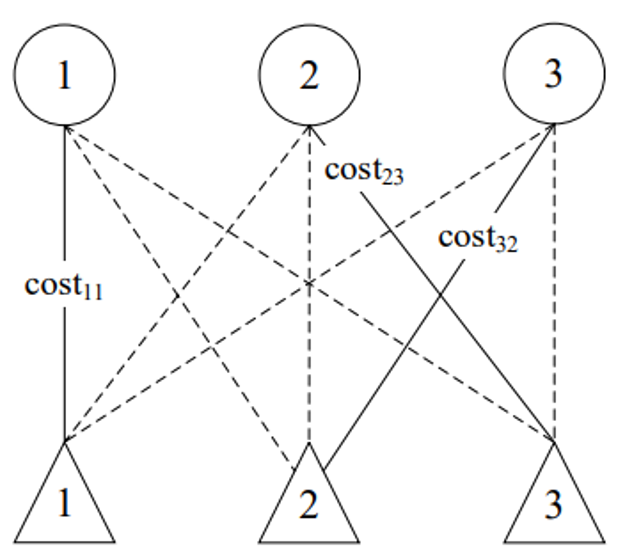
\includegraphics[width=0.4\textwidth]{fig3.1.png}
  \caption{Esquema general del grafo bipartito del problema de programación de vehículos en tiempo real. (Guan et al., 2023)}
  \label{fig:mi_imagen}
\end{figure}

Para resolver este problema, los autores transforman el modelo en un problema de correspondencia en grafos bipartitos ponderados. En esta representación, se presenta un grafo cuyas aristas se tazan entre dos conjuntos de nodos, un conjunto de nodos representa los vehículos disponibles, y el otro conjunto representa las demandas de transporte de los pasajeros. Las aristas entre estos nodos están ponderadas con el costo asociado a cada asignación (considerando factores como distancia y capacidad). El objetivo es encontrar la correspondencia óptima entre vehículos y demandas, minimizando el costo total. En otras palabras, se busca encontrar el conjunto de aristas tal que cada nodo esté conectado exactamente con un nodo del otro conjunto, de forma que se minimice el costo (emparejamiento máximo).

Para implementar este modelo se utiliza el algoritmo de Kuhn-Munkres, también conocido como el algoritmo húngaro. Este algoritmo ajusta iterativamente las correspondencias hasta encontrar la solución que minimiza el costo total, garantizando que cada demanda sea asignada al vehículo más adecuado, teniendo en cuenta las restricciones de capacidad y los tiempos de desplazamiento. Esto lo convierte en una solución eficiente y adecuada para escenarios en los que las decisiones de asignación deben tomarse en tiempo real.

El estudio compara los resultados obtenidos con el algoritmo de Kuhn-Munkres frente a un enfoque heurístico, que asigna vehículos a las demandas de manera local e inmediata. Aunque el método heurístico es más rápido, no garantiza una solución óptima global, ya que no evalúa las interacciones entre todas las decisiones de asignación. Por el contrario, el algoritmo de Kuhn-Munkres ofrece una solución óptima global al considerar todas las posibles asignaciones de forma conjunta. En el caso de estudio presentado, el uso de este algoritmo permitió reducir el costo operativo del sistema de 195.34 CNY a 177.67 CNY por viaje, optimizando el uso de los vehículos y minimizando el tiempo que los autobuses permanecen inactivos.

Este trabajo es de gran relevancia para el problema de optimización del despacho de autobuses de interés, ya que la estructura básica del problema es similar, realizar una asignación teniendo en cuenta factores como la demanda, la diversidad de tipos de vehículos, junto restricciones de capacidad y tiempo típicas en cualquier problema de este tipo. La idea de implementar un sistema de reservas en tiempo real, similar al propuesto por Zhou et al., podría aplicarse para mejorar la eficiencia del sistema en Montería, ajustando la asignación de autobuses según la demanda real de los pasajeros y reduciendo los costos operativos. De allí parte otro punto particularmente interesante, la posibilidad de usar grafos bipartitos para modelar la relación entre las cabeceras de las rutas y la demanda de pasajeros. Las cabeceras de las rutas podrían representarse como nodos de un conjunto, mientras que las paradas intermedias y los puntos de demanda formarían el otro conjunto. Las aristas entre estos nodos representarían los trayectos que los autobuses podrían realizar, con pesos asociados a los tiempos de viaje, demanda y otros factores operativos. Este modelo facilitaría la optimización de la asignación de autobuses, permitiendo que los vehículos más grandes sustituyan a los más pequeños en momentos de alta demanda.

Sin embargo, una diferencia importante es que el modelo no incorpora una toma de decisiones dinámica en cuanto a que asigna cada tarea o requerimiento de demanda a un bus partículas(nodo) mientras que en el problema a abordar se debe realizar una toma de decisiones dinámica que se adapte a las distintas fluctuaciones en los tiempos de viaje y demanda de pasajeros que suelen ser significativas dada la hora, el día, el mes, e incluso distintas eventualidades como por ejemplo los días festivos. Adaptar el enfoque flexible de este modelo para considerar estas variables adicionales puede ser retador y requeriría un replanteamiento del grafo, sin embargo, esto mejoraría la robustez del modelo y su aplicabilidad a la realidad operativa de la ciudad, permitiendo un despacho de autobuses más preciso y eficiente que es el fin último.

\subsection*{Artículo 4}

Es de utilidad entender también \textit{“A Data-Driven and Optimal Bus Scheduling Model With Time-Dependent Traffic and Demand”} publicado por Wang et al. (2017) en la revista IEEE Transactions on Intelligent Transportation Systems \parencite{wang2017}. El objetivo de este es aplicar parámetros como el tráfico o la demanda a un problema de despacho de vehículos, para así minimizar el tiempo de espera de los pasajeros. En el modelo que proponen los autores, se toman los siguientes conjuntos: las estaciones que debe recorrer el bus, los pasajeros, la cantidad de buses a disposición y el número de intervalos con los que se cuenta para despachar un bus. Además, hacen uso de los siguientes parámetros: demanda de la ruta para cada franja de tiempo, el tiempo de salida del primer bus, el tiempo de salida del último bus, el tiempo de viaje esperado para ir de una estación a otra en un intervalo, la capacidad de los buses y la cantidad de buses que se encuentran en una estación, entre otros. Así pues, se intenta llegar al valor óptimo de las siguientes variables de decisión: tiempo de salida de un bus de una estación, tiempo de llegada de un bus a una estación, bus al que cada pasajero se monta y el tiempo de espera de cada pasajero. 

Como dentro de los datos de los autores no se encuentra el tiempo de espera individual de cada pasajero, estos asumen lo siguiente: el tiempo de espera de los pasajeros sigue una distribución de probabilidad empírica que sólo depende de la ruta en cuestión (pues diferentes rutas pueden tener diferentes tiempos de espera dependiendo de la política usada). Las capacidades de pasajeros de cada bus le exigen al modelo disponer de restricciones que garanticen que dicha capacidad no sea sobrepasada. Para esto, se toman en cuenta las estaciones en la que los diferentes pasajeros ingresan y salen de un bus. Se asume pues que, si un bus se encuentra en su capacidad máxima al llegar a una estación, los pasajeros de esta deben esperar al siguiente bus para poder transportarse. Entonces, el modelo anterior se resuelve como un MIP (Mixed-Integer Programming) usando el optimizador CPLEX. Cabe resaltar que el modelo se centra también en la eficiencia computacional, por lo que sus resultados están en función del tiempo que le tomó al software encontrar el óptimo.

Así pues, de los elementos mencionados, cabe resaltar aquellos que resultan de mayor aplicabilidad a la problemática a tratar. En los conjuntos y variables se encuentran grandes semejanzas, con la única excepción siendo el tráfico al momento que un bus sale de una estación a otra. En lo que compete a la problemática del presente, no se contemplan estos cambios en el tráfico. Es también interesante la propuesta de Wang et al. de tomar el tiempo de espera de los pasajeros como una distribución de probabilidad \parencite{wang2017}, ya que nosotros tampoco contamos con la hora de llegada exacta de cada pasajero. Lo anterior permite transformar el modelo a uno que no busca directamente satisfacer la mayor cantidad de demanda posible, sino minimizar el tiempo de espera de cada pasajero. Al intentar que cada persona espere el menor tiempo posible para que pase un bus, se minimiza también la probabilidad de que alguno de estos abandone la estación (dejando así demanda sin cumplir). Además, resultan de utilidad las variables que representan la cantidad de buses en cada estación para evitar los desplazamientos sin pasajeros (que no generan valor). También es de interés que el modelo de \textit{“A Data-Driven and Optimal Bus Scheduling Model With Time-Dependent Traffic and Demand”} es un MIP, cosa que aplica de igual forma para el modelo que presentaremos más adelante.


\subsection*{Artículo 5}

Resulta de interés detallar el paper titulado \textit{“Vehicle Dispatch and Route Optimization Algorithm for Demand-Responsive Transit”} publicado por Guan et al. (2022) en la revista Processes \parencite{guan2022}. En este primero se ejecuta un modelo de despacho de vehículos estático para establecer las horas en las que cada bus empieza su ruta. El objetivo es encontrar las rutas que deben ser recorridas de forma que se minimice el kilometraje que recorre cada vehículo. Se cuenta entonces con restricciones como: todas las estaciones con demanda deben ser atendidas; la distancia que recorre un bus no puede sobrepasar una distancia máxima (que entra como parámetro); todo vehículo que sale del patio de origen eventualmente debe volver; y que un bus no puede recorrer más de un número determinado de estaciones. 

Luego, en el trascurso de la operación se ejecuta un segundo modelo, pero esta vez de un despacho dinámico. En cuanto a este segundo modelo, los autores tienen como variables de decisión el orden en el que se recorren las estaciones y la hora de salida/llegada a cada una de estas. La intención principal es reducir la variación en la distancia total que recorren los buses en este nuevo modelo en comparación con lo que recorrían en el modelo inicial (el de despachos estáticos). Así pues, ahora se tienen dos conjuntos de estaciones: aquellas que obligatoriamente deben ser recorridas y aquellas que son opcionales. Se menciona también como restricción que toda estación visitada debe ser abandonada. Se incluye también una variable que explica el tiempo que tarda un bus en arrancar después de detenerse en una estación. Además, se tiene que la cantidad de pasajeros en un bus no puede sobrepasar su capacidad (que es la misma para todos).

El despacho estático es un modelo de programación lineal entera, por lo que los autores aplican un algoritmo genérico basado en estrategia LNS para resolverlo. En cuanto al dinámico, mencionan que aplica un algoritmo de planeación preciso que se aplica sobre la ruta inicial y continuamente la actualiza. Los supuestos que sigue el modelo son: cada estación solo puede tener una solicitud y, en caso contrario, estas solicitudes se subdividen como si fueran otras estaciones (con la misma ubicación geográfica); el principio y fin del recorrido de un bus es en el centro de distribución; la distancia entre estaciones es la más corta posible; sin importar la congestión de las vías, los vehículos viajan a la misma velocidad.

Entonces, la investigación aplica una integración de dos fases que mejora y facilita la implementación de un sistema de despachos dinámico. Es de especial interés este dinamismo, ya que brinda flexibilidad a la hora de responder frente a imprevistos. También permite detectar anomalías en los servicios, lo que a su vez facilita la tarea de reducirlas o, en caso de ser posible, eliminarlas. Para el propósito de nuestra investigación resulta especialmente útil el supuesto de que los buses empiezan y finalizan en un centro de distribución (pues lo mismo aplica para nuestro modelo). También existe la posibilidad de complejizar más la solución, añadiendo por ejemplo un subíndice a la capacidad para que esta dependa del bus particular.

\subsection*{Artículo 6}

Otros aspectos que resultan interesantes de analizar son el modelo y solución planteado en  \textit{“A model for the periodic optimization of bus dispatching times”} publicado por Gkiotsalitis (2020) en Applied Mathematical Modelling \parencite{gkiotsalitis2020}. En este se trabaja sobre datos obtenidos de la línea 302 de buses en Singapur. Su objetivo principal es el ofrecerles flexibilidad a los planeadores al permitirles evaluar y ajustar la planeación de los buses a lo largo de una operación. El autor parte del conjunto de paradas y del conjunto de rutas en dicha línea. Un concepto central que se implementa en el modelo es el de la planeación de la hora de salida de los buses restantes justo antes del despacho de cada bus. Es decir, al momento inicial se calcula la programación del despacho de buses. Justo antes de que parta el segundo bus, se ejecuta de nuevo la programación, pero esta vez tomando el primer bus como el momento cero. Esta iteración se repite entonces para cada bus con el que se cuenta en cada ruta. 

Las variables principales del problema son: la hora original programada para cada viaje, el tiempo objetivo entre la salida de dos buses, el tiempo de permanencia de un bus en cada estación, el tiempo de viaje entre dos estaciones y un factor de peso que se le asigna a cada estación en base a su relevancia. La función objetivo entonces se resume a reducir el cuadrado de la diferencia entre el momento en el que fue programado un viaje y su valor objetivo. Los supuestos empleados fueron: las llegadas de los pasajeros a las estaciones son aleatorias; todos los pasajeros en una estación pueden ser atendidos por el primer bus que pase; entre más pasajeros se suban a un bus en una estación, mayor es el tiempo de permanencia de dicho bus en dicha estación; los tiempos de permanencia son lo suficientemente pequeños como para que ningún pasajero pueda llegar mientras un bus está en una estación. 

Para solucionar el problema, el autor hace uso de aproximaciones del gradiente para aproximar la solución de despachos. Esta solución es considerablemente más rápida que las optimizaciones exactas calculadas con programación cuadrática. Entonces, si bien la solución que se presenta en dicho modelo no es exacta, “la brecha es lo suficientemente despreciable en escenarios realistas de operación de autobuses” \parencite{gkiotsalitis2020}.

Del modelo presentado anteriormente existen cosas a remarcar que resultan de especial utilidad para este tipo de trabajos. La primera y más importante es el cómo trabaja iterativamente al momento de cada despacho para recalcular y comparar las horas de salida programada para las rutas posteriores. Al momento de programar la salida de buses, existen variables imposibles de predecir con exactitud (como el tráfico) que, si bien no se contempla directamente en este modelo, su solución permite reaccionar a pequeñas variaciones en este para garantizar una operación óptima de la flota de buses. Sin embargo, uno de los aspectos que es explorado en el modelo de Gkiotsalitis que no es de nuestro interés es el del tiempo de permanencia de un bus en una estación. Al no contar con datos históricos que nos den indicios del comportamiento de esta variable para nuestro caso particular, resulta despreciable y puede ser ignorada por completo en nuestro modelo.

\subsection*{Artículo 7}

El artículo \textit{“Vehicle dispatching in modular transit networks: A mixed-integer nonlinear programming model”} (Pei et al., 2021) introduce un enfoque novedoso para la optimización de vehículos en redes de tránsito modular (MTNS) \parencite{pei2021}. El objetivo principal de este estudio es maximizar la eficiencia operativa de un sistema de transporte público mediante el uso de vehículos modulares, los cuales tienen la capacidad de ajustar su tamaño en tiempo real al acoplar o desacoplar módulos de manera dinámica a lo largo de la ruta. Este modelo se presenta como una alternativa a los sistemas tradicionales de transporte público, en donde los vehículos tienen una capacidad fija, lo que no permite adaptarse bien a la demanda de pasajeros, provocando un desajuste entre la oferta y la demanda, con largas esperas de los pasajeros cuando la demanda excede la capacidad del vehículo y bajos niveles de ocupación cuando la demanda es menor que la capacidad del vehículo.

La formulación desarrollada por Pei et al. para optimizar la estrategia de despacho de vehículos y los itinerarios de los pasajeros se basa en un modelo de programación no lineal de enteros mixtos (MINLP) que busca optimizar dos componentes clave: los costos operativos del sistema de transporte y los tiempos de viaje de los pasajeros (también modelado como costos). Por lo tanto, la función objetivo del modelo busca un equilibrio entre minimizar los costos operativos, que incluyen la distancia recorrida por los vehículos modulares y el tiempo de espera de los pasajeros. De este modo, se maximiza la eficiencia del sistema optimizando la frecuencia de despacho de vehículos y la capacidad de cada vehículo.

La estructura del modelo incluye varias restricciones para establecer el funcionamiento del sistema. En primer lugar, está la capacidad de los vehículos, que limita la cantidad de pasajeros que cada vehículo puede transportar en los diferentes tramos de la red de forma que no supere su capacidad. En segundo lugar, se garantiza la conservación de los vehículos, es decir, que el número de vehículos que llegan a una estación debe ser igual al número que sale, para evitar desbalances en la capacidad a lo largo de la red. Asimismo, se incluye una restricción de flujo de pasajeros, asegurando que cada pasajero pueda completar su viaje, ya sea mediante una ruta directa o con transbordos entre vehículos modulares. Finalmente, la unicidad del tipo de vehículo por enlace asegura que solo un tipo de vehículo modular opere en cada segmento de la red, lo cual simplifica las operaciones de tránsito (esto es un supuesto del problema dado que no necesariamente la operación real funciona de esta forma).

El principal desafío del modelo es su complejidad inherente debido a la interacción de las decisiones sobre la frecuencia de los vehículos y la capacidad modular en cada enlace. Esto se traduce en un problema no lineal de difícil resolución. Para resolverlo de manera eficiente, el artículo propone una reformulación lineal que permite resolverlo usando herramientas estándar de programación lineal entera mixta (MILP). Esta formulación permite que el problema sea más manejable desde el punto de vista computacional, obteniendo soluciones cercanas al óptimo original del MINLP.

Para resolver el modelo linealizado, se utiliza el optimizador comercial Gurobi. El modelo se prueba en dos casos de estudio en China: un sistema de transporte suburbano y un sistema de autopista. Los resultados de estos experimentos muestran que el sistema de tránsito modular propuesto es capaz de reducir de manera significativa tanto los costos operativos como los tiempos de viaje de los pasajeros en comparación con los sistemas de vehículos de capacidad fija (FSBS) y con los sistemas de transporte privado (PCS). Este hallazgo destaca la capacidad del sistema modular para ajustarse a la variabilidad de la demanda y optimizar la asignación de recursos, lo que se traduce en un mejor rendimiento en comparación con los sistemas de transporte convencionales.

El trabajo de Pei et al. se apoya en diversos estudios sobre la optimización de redes de transporte. El artículo hace referencia a investigaciones previas como las de (Daganzo, 2010) \textcite{daganzo2010} y (Ouyang, et.al 2014) \textcite{ouyang2014}, quienes exploraron la optimización de rutas y frecuencias en sistemas de transporte público para minimizar los costos. Además, se apoya en investigaciones recientes sobre vehículos modulares, como el estudio de (Chen et.al. 2019) \textcite{chen2019}, en donde se investigó el uso de vehículos modulares en sistemas con alta congestión de tráfico. La aportación distintiva de este modelo reside en la integración de la modularización de los vehículos en una red completa de tránsito, permitiendo ajustes tanto en la frecuencia como en la capacidad en función de las condiciones de demanda.

El modelo incluye varias simplificaciones para facilitar su implementación. Asume que la demanda de pasajeros es constante a lo largo del tiempo y que las estaciones tienen suficiente capacidad para almacenar los módulos de vehículos, lo que permite ajustar fácilmente la capacidad de los vehículos. Además, no se considera la congestión del tráfico, ya que se supone que el impacto en la red es mínimo. Solo se permite un tipo de vehículo modular por enlace, lo que simplifica el problema computacional, y el tiempo de espera de los pasajeros se estima como la mitad del intervalo de despacho, lo cual es una aproximación común, pero puede no reflejar con precisión las complejidades reales de la espera y transferencia de pasajeros. Estas simplificaciones ayudan a hacer el modelo más manejable, aunque limitan su aplicabilidad en escenarios más realistas.

El enfoque presentado en el modelo de redes de tránsito modular tiene ciertas particularidades que, si bien no son directamente aplicables al sistema de autobuses de Montería, sí ofrecen ideas útiles en cuanto a la gestión de la capacidad y la optimización de frecuencias, lo que puede ser adaptado a sistemas con características distintas. Aunque Montería no cuenta con vehículos modulares como los descritos en el artículo, la noción de ajustar la frecuencia de los despachos en función de la demanda real o proyectada en intervalos predefinidos, con autobuses más frecuentes en horas pico y menor frecuencia en horas valle, podría ser beneficiosa. Otro aspecto que se podría adaptar es el objetivo del problema, en donde el modelo busca minimizar los costos mediante un ajuste óptimo de las capacidades y frecuencias de los vehículos, lo cual podría configurarse en el problema de interés de forma que busque reducir el costo operativo evitando despachos innecesarios, atenciones a demandas insuficientes, viajes en vacío, entre otros. Finalmente, la idea de que la oferta de transporte debe ajustarse dinámicamente a la demanda es directamente relevante para Montería. Aunque no pueda implementarse con la misma flexibilidad que en el modelo modular, el sistema de Montería podría beneficiarse enormemente de una asignación adaptativa basada en la previsión de demanda de pasajeros en diferentes momentos y días.

\subsection*{Artículo 8}


El artículo “Models for Line Planning in Public Transport” por los autores Ralf Borndorfer, Martin Grötschel y Marc E. Pfetsch \cite{borndorfer2005}, los cuales son profesores de matemática y optimización de la universidad de Berlín, se enfoca en encontrar las frecuencias de los buses en el medio de transporte público para cumplir con la demanda. Donde la empresa transportadora busca minimizar los costos de operación y tiempos cortos en el bus. Para el planteamiento de este problema tiene como base y estrategia para solucionar este problema el uso de matrices de origen-destino de los pasajeros que quieren transportarse de un punto a otro en un tiempo dado.

El primer paso para realizar el cálculo de la frecuencia es determinar las rutas, calles y direcciones por las cuales se van a transportar los buses durante el día. Este hecho se puede usar ya líneas establecidas para reducir la necesidad computacional del problema. El segundo paso en el problema planteado busca encontrar la frecuencia de buses en cada línea satisfaciendo la demanda que se tiene en cada nodo de la matriz. El tercer paso que se tiene que establecer es el hecho de encontrar los tiempos de salida minimizando el tiempo de transferencia y el número de vehículos para satisfacer la demanda. En este artículo, los autores buscan enfocarse en encontrar los elementos del segundo paso donde plantean dos soluciones con modelos lineales con múltiples objetivos. Ambos modelos planteados minimizan la combinación del tiempo total de transporte de los pasajeros y los costos.

El primer modelo que plantean usa dos variables, la primera variable de las líneas a utilizar y la segunda de la cantidad de las rutas de los pasajeros de un nodo a otro. Este modelo retorna una solución no tan cercana al óptimo, pero luego puede ser utilizada; sin embargo, el segundo modelo es más robusto. El segundo modelo también utiliza variables de ruta de pasajeros y en las líneas, pero con restricciones en el uso de las líneas. Para ambos modelos, se permite que los pasajeros cambien las rutas dependiendo del tiempo que se encuentran en el sistema.

Primero se explicarán los elementos utilizados para ambos modelos. El modelo planteado por los autores establece un grafo unidireccional para entender las rutas y las líneas de los buses. Además, indexan el tipo de bus en un mismo parámetro donde se encuentra el nodo de inicio, nodo final, su frecuencia y el tipo de bus ya que tienen la disponibilidad del tipo de bus para esa línea. Además, tienen en cuenta los costos operativos en cada nodo y también la capacidad que se puede tener en cada nodo. No existen demandas negativas, la matriz no es simétrica. Se asume que el pasajero toma la ruta más corta por lo que solo se llegaría una vez a un nodo. Por último, tienen en cuenta la capacidad para cada tipo de bus.

El primer modelo es un modelo que encuentra valores factibles que cumplen con el objetivo, pero no encuentra una solución muy adecuada. Establecen que las soluciones que se pueden obtener son finitas ya que solo se puede llegar a un nodo una única vez. Por esto, la cantidad de nodos en la matriz es el máximo que se puede obtener. El objetivo de este modelo es minimizar el tiempo de los pasajeros y los costos. Esta función objetivo está sujeta a nueve restricciones donde dos son la naturaleza de las variables.

En el presente estudio, se han establecido varias restricciones fundamentales para el modelo de optimización del sistema de transporte. En primer lugar, la restricción de flujo del sistema garantiza que el número de pasajeros en un autobús se mantenga constante en cada instante, ajustando la cantidad de pasajeros a bordo según la demanda en el nodo correspondiente, considerando las subidas y bajadas de pasajeros. La restricción de capacidad del autobús impide que la cantidad de pasajeros que suben durante cada trayecto supere la capacidad máxima del vehículo, evitando así su sobrecarga. Por otro lado, la restricción de utilización de autobuses asegura que todos los autobuses empleados durante el período de análisis deben regresar al sistema al finalizar su recorrido, lo que facilita una gestión eficiente de la flota. La restricción de ruta obligatoria establece que cada ruta debe seguir un trayecto específico hasta un nodo designado, asegurando que se cumplan los requisitos operacionales establecidos. Además, la restricción de no existencia de subtours prohíbe la formación de ciclos o circuitos innecesarios, previniendo recorridos redundantes y mejorando la eficiencia del sistema. La restricción de demanda estipula que no se debe satisfacer una demanda que exceda la capacidad disponible en cada trayecto, garantizando que la oferta no supere la demanda en cada segmento del recorrido. Finalmente, la restricción de frecuencia máxima limita a un máximo de una frecuencia de servicio por cada arco del modelo, con el fin de asegurar una distribución equitativa de los recursos y evitar la sobrecarga en cualquier arco del sistema.

Estas restricciones son fundamentales para la adecuada formulación y solución del modelo de optimización, garantizando que el sistema de transporte opere de manera eficiente y eficaz. El primer modelo permite abordar el problema de manera más manejable mediante la relajación de la restricción de no existencia de subtours. Esta relajación facilita la resolución del modelo, permitiendo que se obtengan soluciones en tiempos polinomiales, lo cual es crucial para manejar problemas de gran escala en un tiempo computacionalmente razonable.

El segundo modelo planteado hace uso de tres variables: el flujo de pasajeros de un nodo a otro por un arco, una segunda variable que muestra si una línea se utiliza o no se utiliza, y la tercera variable que es la frecuencia de la línea. Con estas variables se puede calcular el costo total (costos de establecimiento de ruta y costos de frecuencias) y el tiempo de las personas en transporte, el cual se quiere minimizar. Este modelo cuenta con siete restricciones, las cuales se mencionarán a continuación.

La primera restricción asegura la conservación del flujo dentro del sistema, garantizando que el número de pasajeros en cada nodo coincida con la demanda en ese punto. La segunda restricción establece que la cantidad de pasajeros en cada arco y en cada línea de la matriz no debe exceder la capacidad máxima de los autobuses. Adicionalmente, se incluye una restricción que limita la frecuencia máxima permitida en el sistema para evitar saturaciones. Otra restricción emplea la técnica de la constante gran M para determinar la frecuencia de uso de las líneas, facilitando el establecimiento de esta relación. Finalmente, las últimas tres restricciones se refieren a la naturaleza de las variables, definiendo las condiciones bajo las cuales operan y asegurando la integridad del modelo.

Los autores destacan que este modelo es más sencillo que el primero en el sentido de que facilita la incorporación de nuevas restricciones. Sin embargo, a pesar de esta flexibilidad, el modelo se clasifica como NP-Hard debido a las restricciones impuestas, lo que obliga a utilizar métodos de relajación. Estos métodos implican la activación o desactivación de restricciones para obtener soluciones iniciales, las cuales se ajustan progresivamente para mejorar la solución general.

Ambos modelos utilizan los mismos cinco supuestos fundamentales. El primer supuesto establece que los pasajeros planifican sus viajes según las líneas de transporte predefinidas, mostrando rigidez respecto a la demanda en diferentes áreas. El segundo supuesto indica que las líneas de transporte son simples, es decir, las rutas o calles son bidireccionales, lo que simplifica el movimiento a lo largo de las rutas. El tercer supuesto asume la ausencia de transferencias de pasajeros entre nodos. El penúltimo supuesto establece que el período de estudio óptimo corresponde a un día completo o al período de mayor demanda durante el día. Finalmente, el último supuesto establece que las frecuencias deben ser números enteros, ya que no se pueden utilizar frecuencias continuas en la práctica; estas frecuencias se ajustan luego a los tiempos de las rutas.

El análisis del artículo revela que, aunque se emplean diferentes enfoques, ambos modelos comparten objetivos similares en la resolución del problema. Ambos buscan mantener la conservación de flujos en el sistema, lo que garantiza la estabilidad de este. Además, ambos modelos se enfocan en no exceder la capacidad de los autobuses ni la demanda esperada, evitando así la sobrecarga. También consideran el uso de variables relacionadas con la demanda y las líneas de transporte utilizadas.

El modelo propuesto por Borndorfer et al. \cite{borndorfer2005} ofrece estrategias valiosas para abordar el problema en Montería. Un aspecto clave es la utilización de las líneas de transporte ya establecidas por la empresa, ya que se busca optimizar los tiempos en rutas preexistentes. Asimismo, se mantiene la conservación de flujos en el sistema, asegurando que no se satisfaga una demanda mayor a la capacidad disponible. Finalmente, la restricción de no exceder la capacidad de los autobuses es crucial, dado que, en Montería, con el sistema MoviSinu, la cantidad de autobuses es limitada.

\subsection*{Artículo 9}

Por último, el artículo “Robust timetable optimization for bus lines subject to resource and regulatory constraints” \cite{gkiotsalitis2019} presenta un enfoque innovador para la optimización de horarios de autobuses que tiene en cuenta la incertidumbre inherente en los tiempos de viaje y la demanda de pasajeros. El objetivo principal es desarrollar un método que genere horarios robustos que puedan mantener un buen desempeño incluso en escenarios de peor caso, es decir, cuando se enfrentan a interrupciones significativas en los tiempos de viaje y la demanda de pasajeros. Para lograr esto, los autores proponen un modelo que utiliza conjuntos de incertidumbre en lugar de distribuciones de probabilidad, eliminando la necesidad de ajustar distribuciones para cada enlace o demanda, algo que es laborioso y, a menudo, inexacto. El modelo busca minimizar las pérdidas operativas bajo los escenarios más adversos.

Este trabajo se apoya en investigaciones previas, como las de Ibarra et al. (2015), que destacaron la importancia de utilizar datos de operación histórica para enfrentar la incertidumbre en los tiempos de viaje \cite{ibarra2015}. Además, este artículo complementa el enfoque de optimización estocástica que ha sido tradicional en la literatura de planificación de horarios, ofreciendo una alternativa que, en lugar de depender de distribuciones de probabilidad, emplea conjuntos de incertidumbre que pueden cubrir una mayor variedad de escenarios disruptivos.

El modelo se formula como un problema minmax que incorpora un enfoque de optimización evolutiva y programación secuencial cuadrática. La optimización se enfoca en dos objetivos principales: mejorar la regularidad del servicio (minimización de la desviación respecto a los intervalos planificados) y evitar que los tiempos de viaje se prolonguen significativamente más allá de lo previsto, lo que afectaría las operaciones futuras.

El modelo se restringe teniendo en cuenta las limitaciones prácticas, como el tiempo mínimo de descanso requerido para los conductores, el tiempo de recuperación y los límites máximos en los intervalos entre despachos para garantizar un nivel de servicio mínimo. Además, el modelo impone que el tiempo de despacho de los viajes no debe desviarse significativamente del plan original y que el tiempo de finalización de cada viaje no puede exceder un cierto límite.

Para resolver el problema se utiliza un algoritmo genético combinado con programación secuencial cuadrática, en el cual se generan soluciones robustas a lo largo de varias generaciones de poblaciones, evaluando el rendimiento bajo los escenarios más adversos de tiempos de viaje y demanda de pasajeros. La solución se valida en una línea circular de autobuses en Singapur, donde se observa una mejora en la regularidad del servicio del 5.17\% y una reducción del 6.87\% en los tiempos de viaje excesivos, comparado con los horarios planificados originalmente.

Una de las grandes contribuciones de este trabajo es su capacidad para generar horarios que se desempeñan bien en escenarios de peor caso sin requerir estimaciones precisas de la probabilidad de las perturbaciones. Los autores argumentan que los horarios generados por enfoques que dependen de distribuciones de probabilidad tienden a fracasar cuando las perturbaciones reales caen fuera de las regiones de alta probabilidad de esas distribuciones, lo que motiva el enfoque robusto basado en incertidumbre presentado aquí.

De hecho, este enfoque podría ser interesante de incluirlo como una posible forma para manejar la estocasticidad de la demanda, dado que esta es difícil de predecir con precisión, por lo que no es viable depender de estimaciones precisas de probabilidades. Adicionalmente, el hecho de que se pueda tener en cuenta tanto la operación regular como la operación enfrentada a los escenarios menos favorables permitiría que el agente despachador pueda tomar decisiones dinámicas en dichas situaciones, aliviando el impacto que estos eventos puedan tener en la operación del sistema. Sin embargo, existen claras limitaciones que hacen que este enfoque no sea directamente aplicable, siendo la principal el acceso a un suministro de datos históricos, dado que las empresas no han logrado establecer una infraestructura que les facilite realizar el registro de los históricos de datos de forma eficiente.

\section{Planteamiento del Problema}

En el contexto de la movilidad urbana, la eficiencia del transporte público es un factor determinante no solo para la calidad de vida de los ciudadanos, sino también para la sostenibilidad de las ciudades. Un sistema de transporte eficiente no solo minimiza los tiempos de espera y mejora la experiencia del usuario, sino que también maximiza el aprovechamiento de los recursos disponibles, contribuyendo a una menor congestión vehicular, menor contaminación y una optimización en el uso del espacio urbano.

En la ciudad de Montería, Córdoba, el sistema de transporte público enfrenta desafíos significativos, especialmente en la programación y despacho de buses. Actualmente, Montería cuenta con 21 rutas de transporte público, operadas por varias empresas: Metrosinu; Monteria Express, Sinumovil; Monteriana Movil. Cada ruta tiene dos cabeceras, que sirven como puntos de partida para los recorridos en ambos sentidos (por ejemplo, Mocarí-Panzenu y Panzenu-Mocarí). El recorrido de una cabecera a la otra se conoce como un sentido de la ruta, por lo que debe ser claro que todas las rutas presentas dos sentidos(puede entenderse como idea y vuelta) no necesariamente paralelos, por lo que su comportamiento en cuanto a demanda y tiempos de recorrido serán independientes y únicos para cada sentido a pesar de ser la misma ruta. 

La empresa cuenta con un único tipo de bus con capacidad de 52 pasajeros. Los buses pueden ser asignados desde cualquiera de las dos cabeceras, y cada sentido de la ruta está compuesto por tramos o "arcos" que marcan el recorrido entre puntos clave de la ciudad. Sin embargo, estos arcos son utilizados únicamente de forma interna por las empresas como guía, ya que el sistema no cuenta con paraderos fijos ni información detallada sobre características o registros específicos en estos subtramos, lo que limita la precisión en la planificación operativa obligando a trabajar directamente desde los sentidos de cada ruta. Cabe aclarar que estos buses no inician su operación desde las respectivas cabeceras, sino que todos al salir de operación son guardados en un patio común, desde donde son despachados al momento que se requieran en las cabeceras para iniciar sus nuevos recorridos, lo que claramente tiene implícito un tiempo en transito de patio a cabecera al iniciar o reanudar la operación, y de cabecera a patio al finalizarla.

Cada empresa operadora recibe mensualmente una cantidad máxima de vehículos para operar en las rutas, teniendo en cuenta ambos sentidos. Esto significa que no todas las rutas pueden ser cubiertas de manera simultánea, y que existe un límite en la cantidad de buses que pueden circular en cada ruta. Esta restricción obliga a las empresas a gestionar de forma óptima los vehículos disponibles para satisfacer la mayor demanda posible a lo largo del día. El problema principal radica en que la programación actual del despacho de buses se basa en un método manual y poco robuzto, que no se ajusta de manera eficiente a las necesidades del servicio, a las fluctuaciones de la demanda, a la capacidad de los buses, eventualidades de los diferentes días y horas de la operación, imprevistos, entre otros aspectos típicos de la operación de un servicio de transporte público.

Por lo tanto, el problema que se quiere atacar es la ineficiencia en la programación del despacho de buses en el sistema de transporte público de Montería. Actualmente, las decisiones sobre el despacho de buses se toman mediante un procedimiento rudimentario que, aunque permite mantener la operación funcional, no optimiza la distribución de los recursos ni maximiza la atención a los pasajeros. Este proceso manual se estructura en dos pasos principales:

\begin{enumerate}
    \item \textbf{Distribución inicial de buses:} Los buses se asignan equitativamente entre los dos sentidos de cada ruta, salvo que los tiempos de tránsito entre cabeceras difieran significativamente, en cuyo caso se ajusta la proporción de buses en cada sentido.
    \item \textbf{Cálculo de intervalos de despacho:} A partir del tiempo de tránsito promedio entre cabeceras, se calcula un intervalo de despacho para cada hora de operación (de 5:00 a.m. a 9:00 p.m.). Este intervalo se determina dividiendo el tiempo de tránsito por el número de buses disponibles, lo que establece la frecuencia de despacho desde cada cabecera.
\end{enumerate}

La operación actual le ha permitido a la empresa alcanzar un IPK de 0.7 pasajeros por kilómetro por ruta en promedio. Si bien este enfoque básico permite una operación inicial con cierta regularidad, los intervalos de despacho se desajustan una vez los buses comienzan a circular. Esto ocurre debido a la variabilidad en los tiempos de retorno de los vehículos, que dependen de factores como el tráfico y las condiciones específicas de la ruta. Los buses solo están disponibles para ser despachados una vez completan su recorrido, lo que provoca desfases respecto al intervalo planificado inicialmente.

Además de estos problemas operativos, el método actual no considera un factor clave: la demanda de pasajeros. La cantidad de usuarios varía significativamente según la hora del día, el día de la semana e incluso factores estacionales o eventos imprevistos que son cotidianos en este tipo de actividad como se mencionó anteriormente. Al no tomar en cuenta estos factores, el sistema actual puede asignar demasiada capacidad en momentos de baja demanda, o insuficiente capacidad en las horas pico. Esto genera tiempos de espera prolongados y una distribución ineficaz de los recursos, lo que afecta tanto la experiencia de los usuarios como los costos operativos de las empresas.

No obstante, también se presentan importantes limitaciones con los datos históricos que la infraestructura de información de la empresa ha logrado recolectar. Por un lado, se conoce un registro de ventas históricas registradas a partir del sistema de torniquetes de los respectivos buses. Estos datos no corresponden a la demanda ya que no se esta teniendo en cuenta aquella demanda perdida, esto es aquellas personas que por ejemplo tuvieron que esperar mucho tiempo y decidieron optar por un medio de transporte alternativo, o situaciones similares. Adicionalmente, los registros de pasajeros están sesgados respecto al sentido de la ruta donde se presento esta demanda dado que son los conductores los que al completar un trayecto deben configurar el dispositivo para iniciar los registros en el otro sentido de la ruta, sin embargo, por información suministrada por la empresa se conoce que estos suelen fallar en este proceso omitiéndolo o realizándolo de forma incorrecta, por lo que aunque estos registros si corresponden efectivamente a la ruta informada en el dato, el sentido no necesariamente es el correcto, por lo que la información de ventas y tiempo de ruta de los trayectos de los diferentes sentidos puede estar sesgada. Por lo tanto, debe ser claro que, dada la naturaleza de los datos, el problema debería ser planteado de forma determinística ante la poca información para poder incluir estocasticidades.

Abordar este problema es crucial para mejorar la eficiencia operativa y garantizar un servicio de transporte público más confiable y ajustado a las necesidades reales de los usuarios. La ineficiencia en la programación de los despachos no solo afecta a los pasajeros, quienes enfrentan tiempos de espera irregulares, sino que también tiene un impacto directo en los costos y la sostenibilidad del sistema. La sobreoferta de buses en horarios de baja demanda genera un uso innecesario de combustible y recursos perdiendo incluso recorridos enteros por viajes en vacío, mientras que la suboferta en horas pico produce congestión y frustración entre los usuarios, lo que puede desincentivar el uso del transporte público en favor de opciones privadas menos sostenibles. Esto último genera además pérdidas a la empresa, pues es demanda que se deja de atender. Un pasajero que espera mucho tiempo el paso de un bus puede buscar alternativas como el uso de otro servicio público, lo que al largo plazo llega a afectar incluso a la imagen de la organización.

Un despacho ineficiente también contribuye al desgaste prematuro de los vehículos, incrementando los costos de mantenimiento y reduciendo la vida útil de la flota. Estos factores afectan negativamente la sostenibilidad económica y ambiental del sistema, dificultando la posibilidad de ofrecer un servicio de calidad y competitivo frente a otras alternativas de movilidad.

Como los buses proveen una mejor eficiencia en utilización de recursos que los autos privados, el número de vehículos en las vías puede ser reducido considerablemente \cite{wang2017}. Con más y más buses en circulación, los pasajeros disfrutan de un servicio de mayor calidad producto de menores tiempos de espera y menos transbordos en trayectos largos. Sin embargo, esto impone una carga en los proveedores de dicho servicio en cuanto al controlar el presupuesto de las operaciones. 

Por tanto, es esencial diseñar una estrategia de despacho de buses robusta que considere tanto la demanda de pasajeros como los diferentes factores operativos que componen al sistema, con el objetivo de optimizar la atención a los usuarios y maximizar la eficiencia en el uso de los recursos. Este enfoque no solo permitirá mejorar la calidad del servicio, sino que también reducirá los costos operativos y contribuirá a un sistema de transporte más sostenible a largo plazo.

\section{Justificación}

El sistema de transporte público de Montería enfrenta un reto significativo en la programación y despacho de sus buses, lo que afecta tanto a la eficiencia operativa como a la satisfacción de los usuarios. Actualmente, la asignación de buses se realiza de manera manual y con información limitada, lo que no permite ajustar el servicio a las variaciones en la demanda de pasajeros ni responder de forma efectiva a las fluctuaciones operativas. Esta falta de precisión conlleva un uso ineficiente de los recursos, resultando en tiempos de espera prolongados para los pasajeros, sobreoferta de buses en momentos de baja demanda y suboferta en horas pico, afectando directamente la experiencia del usuario y los costos operativos de las empresas.

Desde el punto de vista económico, un sistema de transporte público mal gestionado genera costos innecesarios para las empresas operadoras, ya que la falta de optimización en la asignación de vehículos incrementa el consumo de combustible y el desgaste prematuro de los buses, reduciendo su vida útil. Estas ineficiencias también repercuten en la sostenibilidad del sistema, ya que una menor rentabilidad pone en riesgo la continuidad y calidad del servicio a largo plazo.

El desarrollo de un modelo de optimización del despacho de buses permitirá maximizar el uso de la flota disponible, adecuando la oferta de vehículos a la demanda real de los pasajeros. Al optimizar la distribución de los buses, se espera reducir los tiempos de espera, mejorar la satisfacción de los usuarios y minimizar el número de recorridos con baja ocupación. Este enfoque no solo incrementará la eficiencia operativa del sistema, sino que también contribuirá a reducir el impacto ambiental al minimizar el número de viajes en vacío y el consumo de recursos innecesarios.

Adicionalmente, la implementación de un sistema de programación basado en datos precisos proporcionará una mayor capacidad de reacción frente a las condiciones operativas, permitiendo que las empresas operadoras ajusten la frecuencia de los despachos en tiempo real según la demanda y las condiciones del tráfico. En última instancia, este modelo contribuirá a la sostenibilidad económica, social y ambiental del sistema de transporte público en Montería, haciéndolo más competitivo frente a otras alternativas de movilidad y alineado con los objetivos de movilidad urbana sostenible.

\section*{Objetivos}

\subsection*{General}

Desarrollar un modelo de optimización para la programación y despacho de buses en el sistema de transporte público de Montería, que permita una asignación eficiente de los recursos disponibles, maximizando el nivel de servicio de los usuarios.

\subsection*{Especificos}

\begin{itemize}
    \item Diseñar un modelo de optimización que integre la demanda dinámica de pasajeros a lo largo del día y de la semana, considerando factores como la variabilidad en los flujos de usuarios, la capacidad de los vehículos y los tiempos de tránsito, con el objetivo de optimizar la asignación de buses en ambas direcciones de cada ruta.
    \item Establecer un sistema de despacho basado en intervalos ajustables que permita adaptar la frecuencia de salida de los buses de manera automática, teniendo en cuenta factores operativos como las condiciones del tráfico, los tiempos de trayecto y la disponibilidad de vehículos en cada momento de la operación.
    \item Validar el modelo propuesto mediante simulaciones que comparen el desempeño del sistema optimizado frente al sistema actual, evaluando métricas clave como la reducción de tiempos de espera para los usuarios, el incremento en la ocupación de los buses y la eficiencia en el uso de los recursos.
\end{itemize}

\section{Bibliografía}
\printbibliography % Esto imprime la sección de referencias

\end{document}

